% !TEX TS-program = pdflatex
% !TEX encoding = UTF-8 Unicode
% !TEX spellcheck = es_CL

% This is a simple template for a LaTeX document using the "article" class.
% See "book", "report", "letter" for other types of document.

%\documentclass[preview=true, landscape]{standalone}
\documentclass[landscape]{article}

%\usepackage{svn-multi}
%\svnidlong
%{$HeadURL$}
%{$LastChangedDate$}
%{$LastChangedRevision$}
%{$LastChangedBy$}
\usepackage[utf8]{inputenc} % set input encoding (not needed with XeLaTeX)
\usepackage[T1]{fontenc}
\usepackage{lmodern}
\usepackage[spanish,es-tabla]{babel}
\spanishdecimal{.}
%%% Examples of Article customizations
% These packages are optional, depending whether you want the features they provide.
% See the LaTeX Companion or other references for full information.

%%% PAGE DIMENSIONS
\usepackage{geometry} % to change the page dimensions
\geometry{letterpaper} % or letterpaper (US) or a5paper or....
\geometry{margin=1.4in} % for example, change the margins to 2 inches all round
% \geometry{landscape} % set up the page for landscape
%   read geometry.pdf for detailed page layout information

\usepackage{graphicx} % support the \includegraphics command and options

% \usepackage[parfill]{parskip} % Activate to begin paragraphs with an empty line rather than an indent

%%% PACKAGES
\usepackage{booktabs} % for much better looking tables
\usepackage{array} % for better arrays (eg matrices) in maths
\usepackage{paralist} % very flexible & customisable lists (eg. enumerate/itemize, etc.)
\usepackage{verbatim} % adds environment for commenting out blocks of text & for better verbatim
\usepackage[subrefformat=parens,labelformat=parens]{subfig} % make it possible to include more than one captioned figure/table in a single float
% These packages are all incorporated in the memoir class to one degree or another...

%\usepackage{amsmath}
\usepackage{mathtools}
\usepackage{amsfonts}


% Paquetes adicionales
\usepackage{siunitx}
\sisetup{load=derived} % loading \si
\usepackage{xcolor}
\usepackage{multicol}
% Paquete titling permite reducir el margen superior
%\usepackage{titling}
%\setlength{\droptitle}{-10ex}
%\usepackage{enumitem}
% agrega la opcion H a las figuras para que queden donde uno quiere
%\usepackage{float}
%\usepackage{microtype}

% Fuentes
% MinionPro
%\usepackage[minionint,textlf,mathlf]{MinionPro}
% Fijar fuente Sans Serif  a Myriad
%\renewcommand{\sfdefault}{Myriad-LF}
%\usepackage[T1]{fontenc}

% Fuente similar a Times New Roman
%\usepackage{tgtermes}
%\usepackage[T1]{fontenc}

%\usepackage{utopia} % Cambia solo la fuente del texto
%\usepackage[urw-garamond]{mathdesign} %Problemas con wrapfig
%\usepackage[utopia]{mathdesign} %Problemas con wrapfig
%\usepackage[charter]{mathdesign} % HERMOSO!!
%\usepackage{fourier} % Problemas con wrapfig
%% Fuente palatino
\usepackage[T1]{fontenc}
\usepackage[sc]{mathpazo}
\linespread{1.05}
%% Similar a palatino pero extendida
%\usepackage{tgpagella}
%\usepackage[T1]{fontenc}
%\usepackage[scaled=0.86]{berasans}
%
%\usepackage{libertine-type1}% NICE!!
%\usepackage{libertine}
%\usepackage[ttscale=0.875]{libertine}
% La fuente typewriter de libertine es fea, asi que hay que cambiarla
%\usepackage{inconsolata}
%\usepackage[scaled=0.83]{beramono}
%\usepackage{DejaVuSansMono}
%\renewcommand\ttdefault{lmtt} % lmtt
%\usepackage[libertine]{newtxmath}
%\usepackage[T1]{fontenc}

%\usepackage[math]{iwona}
%\usepackage{fourier}

%\renewcommand{\sfdefault}{phv}
%\renewcommand{\sfdefault}{lmss} % Fuente por defecto en latex o cmss
% Fuente times
%\usepackage{newtxtext,newtxmath}

%%% SECTION TITLE APPEARANCE
%\usepackage{sectsty}
%\allsectionsfont{\sffamily\mdseries\upshape} % (See the fntguide.pdf for font help)
% (This matches ConTeXt defaults)

%%% ToC (table of contents) APPEARANCE
%\usepackage[nottoc,notlof,notlot]{tocbibind} % Put the bibliography in the ToC
%\usepackage[titles,subfigure]{tocloft} % Alter the style of the Table of Contents
%\renewcommand{\cftsecfont}{\rmfamily\mdseries\upshape}
%\renewcommand{\cftsecpagefont}{\rmfamily\mdseries\upshape} % No bold!

%%% END Article customizations

%%% The "real" document content comes below...
\usepackage[active,pdftex,tightpage]{preview}
%\PreviewEnvironment[]{figure}

\begin{document}

\begin{preview}
%\begin{figure}
% XCircuit output "bloques.tex" for LaTeX input from bloques.ps
\def\putbox#1#2#3#4{\makebox[0in][l]{\makebox[#1][l]{}\raisebox{\baselineskip}[0in][0in]{\raisebox{#2}[0in][0in]{\scalebox{#3}{#4}}}}}
\def\rightbox#1{\makebox[0in][r]{#1}}
\def\centbox#1{\makebox[0in]{#1}}
\def\topbox#1{\raisebox{-0.60\baselineskip}[0in][0in]{#1}}
\def\midbox#1{\raisebox{-0.20\baselineskip}[0in][0in]{#1}}
   \scalebox{1}{
   \normalsize
   \parbox{7.32812in}{
   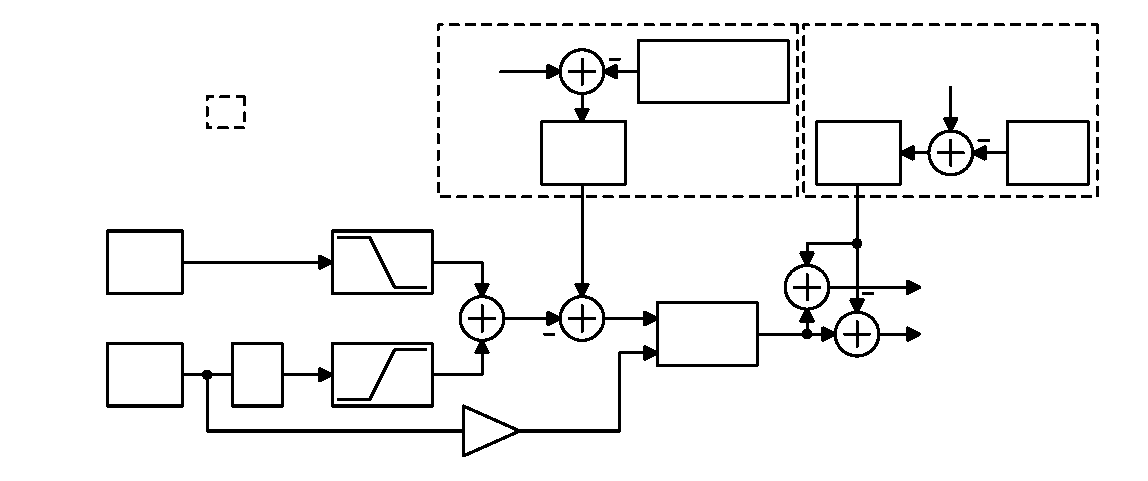
\includegraphics[scale=1]{bloques}\\
   % translate x=649 y=368 scale 0.38
   \putbox{1.60in}{0.60in}{1.20}{\centbox{\midbox{$\int$}}}%
   \putbox{2.44in}{1.60in}{1.20}{\centbox{LPF}}%
   \putbox{2.44in}{0.85in}{1.20}{\centbox{HPF}}%
   \putbox{0.85in}{1.43in}{1.20}{\centbox{\midbox{$\theta_m$}}}%
   \putbox{0.85in}{1.26in}{1.20}{\centbox{\midbox{Accel}}}%
   \putbox{0.85in}{0.51in}{1.20}{\centbox{\midbox{Gyro}}}%
   \putbox{0.85in}{0.68in}{1.20}{\centbox{\midbox{$\dot{\theta}_m$}}}%
   \putbox{3.44in}{1.12in}{1.20}{\centbox{\midbox{$\theta_e$}}}%
   \putbox{4.60in}{0.87in}{1.20}{\centbox{\midbox{PID}}}%
   \putbox{3.79in}{1.56in}{1.20}{\midbox{$\theta_{ref}$}}%
   \putbox{5.62in}{1.64in}{1.20}{\midbox{offset}}%
   \putbox{6.04in}{1.18in}{1.20}{\midbox{PWMA}}%
   \putbox{6.04in}{0.87in}{1.20}{\midbox{PWMB}}%
   \putbox{4.64in}{2.70in}{1.20}{\centbox{\midbox{Encoders}}}%
   \putbox{4.64in}{2.51in}{1.20}{\centbox{\midbox{(velocidad)}}}%
   \putbox{3.77in}{2.08in}{1.20}{\centbox{\midbox{PI}}}%
   \putbox{3.21in}{2.64in}{1.20}{\rightbox{\midbox{$v_{ref}$}}}%
   \putbox{5.60in}{2.08in}{1.20}{\centbox{\midbox{PI}}}%
   \putbox{6.87in}{2.18in}{1.20}{\centbox{\midbox{Gyro}}}%
   \putbox{6.85in}{1.99in}{1.20}{\centbox{\midbox{$\dot{\psi}$}}}%
   \putbox{6.25in}{2.64in}{1.20}{\centbox{\midbox{$\dot{\psi}_{ref}$}}}%
   \putbox{0.96in}{2.29in}{1.20}{\centbox{Ideas}}%
   \putbox{3.08in}{0.22in}{1.20}{\centbox{\midbox{-1}}}%
   } % close 'parbox'
   } % close 'scalebox'
   \vspace{-\baselineskip} % this is not necessary, but looks better

%\end{figure}
\end{preview}
\end{document}
